
\documentclass{article}
\author{Daniel Monjas Miguélez}

\title{Topología II: Ejercicios Resueltos}

\usepackage[spanish]{babel}
\usepackage[utf8]{inputenc}
\usepackage{hyperref}
\usepackage{amsmath}
\usepackage{amssymb}
\usepackage{ textcomp }
\usepackage{ graphicx }
\graphicspath{ {images/} }

\begin{document}
\maketitle

\newpage

\tableofcontents

\newpage

\section{Relación 1}
\subsection{Ejercicio 1}
Sea $I=[0,1]$, y sean $\alpha$ un arco y $\theta$ una aplicación continua tal que $\phi(0)=0$ y $\phi(1)=1$.

Sea 
\begin{equation*}
\left.\begin{array}{c}
H:I\times I\rightarrow X\\
H(t,s)=\alpha((1-s)t+s\phi(t))
\end{array} \right.
\end{equation*}

Ya que $\phi(t)\in I$, el número $(1-s)t+s\phi(t)$ pertenece al intervalo $I$, luego $H$ está bien definida. Por otra parte, dicha aplicación es continua y satisface:
\begin{itemize}
\item $H(t,0)=\alpha(t)$
\item $H(t,1)=\alpha(\phi(t))=\alpha\circ\phi(t)$
\item $H(0,s)=\alpha(0)=\alpha(\phi(0))$
\item $H(1,s)=\alpha(1)=\alpha(\phi(1))$ 
\end{itemize}

, luego existe una homotopía entre $\alpha$ y $\alpha\circ \phi$.

\subsection{Ejercicio 2}
Sea $X\subset \mathbb{R}^n$ un subconjunto estrellado de $\mathbb{R}^n$. Sea $x_0$ el centro de $X$ y sea $\alpha\in\Omega_{x_0}(X)$ un lazo con base el centro de $X$. 

Sea
\begin{equation*}
\left.\begin{array}{c}
H:I\times I\rightarrow X \\
H(t,s)=(1-s)x_0+s\alpha(t)
\end{array}\right.
\end{equation*}

Es calaramente continua y está bien definida, pues para cada $t\in I$, $H(t,s)$ es el segmento que una $x_0$ con $\alpha(t)$, el cual está contenido en $X$, pues al ser $X$ estrellado todo segmento desde el centro de $X$ a un punto de $X$ está contenido en $X$.\\

Para la segunda parte, sean $\alpha, \beta\in \Omega_{p,q}(X)$ con $p,q\neq x_0$. Sean 
\begin{equation*}
\left.\begin{array}{c}
e_1:[0,1]\rightarrow X\\
t\mapsto (1-t)x_0+tp
\end{array} \right.\qquad
\left.\begin{array}{c}
e_2:[0,1]\rightarrow X\\
t\mapsto (1-t)q+tx_0
\end{array} \right.
\end{equation*}

Estos dos segmentos están contenidos en $X$, pues son segmentos que unen el centro del conjunto con otros puntos y por ser $X$ estrellado está bien definido. Como $e_1\in \Omega_{x_0,p}(X)$ y $e_2\in \Omega_{q,x_0}(X)$, entonces $e_1*\alpha*e_2,e_1*\beta*e_2\in \Omega_{x_0}(X)$. Como ya hemos visto que todo lazo del centro del conjunto es homotópico al lazo constante se tiene que
\begin{equation*}
e_1*\alpha*e_2\sim \varepsilon_{x_0}\sim e_1*\beta*e_2\Rightarrow \alpha\sim \beta
\end{equation*}

\subsection{Ejercicio 3}
Veamos que 
\begin{gather*}
\phi_\gamma =\phi_\sigma\Leftrightarrow [\overline{\gamma}*\alpha*\gamma]=[\overline{\sigma}*\alpha*\sigma]\quad \forall [\alpha]\in \Pi_1(X,y) \Leftrightarrow\\
\Leftrightarrow [\overline{\gamma}]*[\alpha]*[\gamma]=[\overline{\sigma}]*[\alpha]*[\sigma] \quad \forall [\alpha] \in \Pi_1(X,y)\Leftrightarrow \\
\Leftrightarrow [\alpha]*[\gamma]*[\sigma]^{-1}=[\overline{\gamma}]^{-1}*[\overline{\sigma}]*[\alpha] \quad \forall [\alpha]\in \Pi_1(X,y)
\end{gather*}
, basta con usar que $[\sigma]^{-1}=[\overline{\sigma}]$. Esto es claro, pues $[\sigma]^{-1}*[\sigma]=[\epsilon_y]=[\overline{\sigma}*\sigma]=[\overline{\sigma}]*[\sigma]$.

De aquí se obtiene pues $[\alpha]*[\gamma]*[\overline{\sigma}]=[\gamma]*[\overline{\sigma}]*[\alpha] \quad \forall [\alpha]\in \Pi_1(X,y)$. Pero de aquí se deduce claramente que $[\gamma*\overline{\sigma}]\in \mathcal{Z}(\Pi_1(X,y))$

\subsection{Ejercicio 4}
Basta con ver que el cono de un espacio $CX$ es $X\times I/\sim$, donde $(x,1)\sim (y,1)$, $\forall (x,y)\in X$.

Observemos que cada $[(x,t)]$ de $CX$ puede conectarse al vértice $[(x,1)]=X\times \{1\}$, mediante el segmento $[(x,(1-s)t+s)]$, $t\in [0,1]$, que esta contenido en $CX$.

Como todo punto de $CX$ se puede unir con $[(x,1)$ entonces se tiene que el cono es un espacio arcoconexo.

\subsection{Ejercicio 5}
$\mathbb{S}^1$ es un retracto fuerte de deformación de $\mathbb{R}^2\backslash \{(0,0)\}$, basta con definir $r(x,y)=(x,y)/\sqrt{x^2+y^2}$. Por tanto $\alpha$ es homotópica a $r\circ \alpha$.

Pero es claro que $r\circ \alpha=\alpha$, luego no es homotópica al lazo constante, en particular la clase de homotopía de $\alpha$ es un generador del grupo fundamental de $\mathbb{R}^2\backslash\{(0,0)\}$ que es $\mathbb{Z}$.

\subsection{Ejercicio 6}
Supongamos que $\mathbb{R}\times [0,\infty)$ es homeomorfo a $\mathbb{R}^2$, entonces 
\begin{equation*}
\mathbb{R}\times [0,\infty)\backslash \{(0,0)\}\cong\mathbb{R}^2\backslash\{f(0,0)\}
\end{equation*}

, pero esto no es posible, pues el grupo fundamental de $\mathbb{R}^2\backslash\{f(0,0)\}$ es $\mathbb{Z}$, mientras que $\mathbb{R}\times [0,\infty)\backslash \{(0,0)\}$, sigue siendo simplemente conexo, luego no pueden ser homeomorfos.

\subsection{Ejercicio 7}
El único caso qeu se va a estudiar es el (f). Los demás se obtiene rápidamente por ser estrellados, o usando la proposición 8.1 de los apuntes de jlopez.

En cuanto al caso $(f)$ basta ver que $f:\mathbb{R}^2\rightarrow \mathbb{R}$, tal que $(x,y)\mapsto z=x^2-y^2$ es una apliación continua. Basta con tomar que el grafo de esta aplicación $G(f)$ que coincide con el paraboloide hiperbólico es homeomorfo al dominio de $f$, el cual sabemos que es simplemente conexo.

\subsection{Ejercicio 8}

\subsection{Ejercicio 9}
$\mathbb{T}=\left\langle (x,y,z)\in \mathbb{R}^3| x=cos\theta\cdot(R+rcos\varphi),\:y=sen\theta\cdot(R+rcos\varphi), z=rsin\varphi\right\rangle$, donde $R$ es la distancia entre el centro del donut y el centro de uno del conducto y $r$ es el radio del conducto.
\begin{figure}[h]
\centering
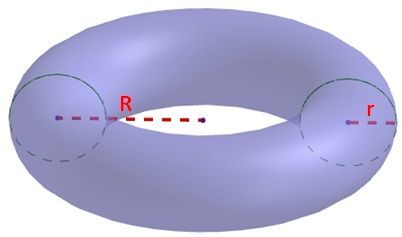
\includegraphics[scale=0.5,width=\textwidth]{toro-volumen.jpg}
\end{figure}

\subsection{Ejercicio 12}
\begin{itemize}
\item Si $f$ es inyectiva, también lo es $f_*$.

Esto no es cierto. Basta tomar la aplicación inclusión como sigue
\begin{gather*}
i:\mathbb{S}^1\rightarrow \mathbb{R}^2\qquad i_*:\Pi_1(\mathbb{S}^1,x)=\mathbb{Z}\rightarrow \Pi_1(\mathbb{R}^2,x)=\{[\varepsilon_x]\}
\end{gather*}
, donde claramente $i_*$ no es una aplicación inyectiva.

\item Si $f$ es sobreyectiva, también lo es $f_*$.
\begin{gather*}
f:\mathbb{R}\rightarrow \mathbb{S}^1\qquad f(t)=(\cos2\pi t,\sen2\pi t)\\
f_*:\{[\epsilon_p]\}\rightarrow \mathbb{Z}
\end{gather*}

y esta aplicación claramente no es sobreyectiva.

\item Si $f$ es biyectiva, también lo es $f_*$.
\begin{gather*}
f:[0,1[\rightarrow \mathbb{S}^1\qquad f(t)=(\cos(2\pi t),\sen(2\pi t))\\
f_*:\{[\varepsilon_p]\}\rightarrow \mathbb{Z}
\end{gather*}

, donde $f$ es claramente continua, inyectiva y sobreyectiva y $f_*$ no puede serlo.
\end{itemize}

\subsection{Ejercicio 13}
\begin{itemize}
\item Claramente $\emptyset$ y $X$ están incluidos en la topología.

\item Por otro lado los abiertos son los conjuntos infinitos, $X$ y $\emptyset$. Claramente la unión de conjuntos abiertos (infinitos) es un conjunto abierto (infinito).

\item Por otro lado supongamos que la intersección de conjuntos abiertos no fuese un conjunto abierto (infinito). Entonces $X\backslash O_1\cap O_2$ sería un conjunto infinito. Pero se tiene que 
\begin{equation*}
X\backslash O_1\cap O_2 = X\backslash O_1\cup X\backslash O_2
\end{equation*}

que es la unión de dos conjuntos finitos, pues sus complementarios son cerrados (finitos) y por tanto la unión de finitos es finita, en contra de la suposición de que el complementario de la intersección no era un conjunto cerrado.
\end{itemize}

Luego hemos deducido que efectivamente, es una topología.\\

Para ver que es arcoconexo, basta tomar dos puntos cuales quiera de $X$ y que por como se ha definido $X$ entre dos puntos cualesquiera habrá exactamente $k$ números naturales distintos de los puntos. Basta con tomar como arco una aplicación tal que 
\begin{gather*}
\alpha:[0,1]\rightarrow X\\
\alpha(t)=\left\lbrace\begin{array}{c}
\alpha(0)=x\\
\alpha(1)=y\\
\alpha(t)=i \quad t=\frac{i}{k+1}\\
\alpha(t)=\infty \quad t\neq \frac{i}{k+1}
\end{array}\right.
\end{gather*}

esta aplicación es continua, pues la preimagen de abiertos es abierto y la preimagen de cerrados es cerrada. Y constituye un arco entre cualesquiera dos puntos de $X$, luego se tiene que $X$ es arcoconexo.

Por otro lado es trivial que es simplemente conexo, pues este espacio es contráctil, y por tanto simplemente conexo.

\subsection{Ejercicio 16}
Supongamos que $\exists\gamma \in \Omega_a(X)$, tal que $\gamma\notin \Omega_a(A)$. Veamos que esto no es posible. 

Si este arco existiera, se tendría que existen valores de $t$ con $t\in I$ tal que $\gamma(t)\notin A$. Pero entonces existe el arco que une $a\in A$ con dichos $\gamma(t)$. De aquí se deduciría que $A\cup \gamma(t)$ sigue siendo arcoconexo, en contra de que $A$ es componente arcoconexa. Por tanto se verifica que $\forall \gamma \in \Omega_a(X)$ se verifica que $\gamma \in \Omega_a(A)$. 

Una vez demostrado esto tendremos que si $\gamma\in \Omega_a(X)$, entonces
\begin{equation}
F_\gamma:\Pi_1(X,a)\rightarrow \Pi_1(X,a)
\end{equation}

es un isomorfismo, pero como todo lazo de $\Omega_a(X)$ está en $\Omega_a(A)$ entonces $\Pi_1(X,a)=\Pi_1(A,a)$ luego por el isomorfismo anterior se tiene el resultado.

\subsection{Ejercicio 17 (Ejercicio 1 Retracciones)}
En primer lugar veamos que es claro que $\mathbb{S}^1\cong I\times \{1/2\}/\sim$.

Con esto claro, vamos a ver que $I\times \{1/2\}/\sim$ es un retracto de deformación de $\mathbb{M}$ y, como es isomorfo a $\mathbb{S}^1$ también lo es $\mathbb{S}^1$. En primer lugar vamos a definir la siguiente aplicación, y veamos que es una retracción:
\begin{gather*}
r:I\times I/\sim \rightarrow I\times \{1/2\}/\sim\\
[(x,y)]\mapsto [(x,1/2)]
\end{gather*}

Esta aplicación está bien definida, pues si $(x,y)$ es un punto que no está en el borde $\{0,1\}\times I$, se relaciona únicamente consigo mismo y por consiguiente la aplicación está definida.

Si el punto $(x,y)$ es del borde anteriormene mencionado, veamos que independientemente de que se cambie el representante de la clase sigue estando bien definido. Esto es cierto, pues si cogemos un representante del borde al aplicarle la imagen nos queda que su imagen es una clase de equivalencia con dos elementos, la imagen del representante y la imagen del putno con el que se relaciona el representante y por consiguiente está bien definido.

En cuanto a la continuidad se puede ver con facilidad que $I\times I \xrightarrow{f} I\times \{1/2\}\xrightarrow{p}I\times\{1/2\}/\sim$ es una aplicación continua, pues al componer $f$ con las proyecciones $p_1$ y $p_2$ nos queda la $Id_I$ y una aplicación constante, luego $f$ es constante y al componer $f$ con la proyección en el cociente es una aplicación continua, luego $r$ es continua.\\

Para la deformación tomamos
\begin{gather*}
F:\mathbb{M}\times [0,1]\rightarrow \mathbb{M}\\
([(x,y)],t)\mapsto [(1-t)(x,y)+tr(x,y)]
\end{gather*}
, es aplicación está bien definida, pues antes de aplicar el cociente claramente el segmento que une dos puntos de $I\times I$ está contenido en $I\times I$ y por tanto la proyección de cualquiera de esos segmentos está en la banda de Möbius.

Por otro lado para ver que es continua, basta ver que en este caso como
\begin{gather*}
p\times 1_{[0,1]}\\
((x,y),t)\mapsto [(1-t)(x,y)+tr(x,y)]
\end{gather*}

es una aplicación continua por ser el producto cartesiano de aplicaciones continuas, entonces nuestra deformación es continua, y por consiguiente $I\times\{1/2\}/\sim$ es retracto de deformación de $\mathbb{M}$ y por tanto $\mathbb{S}^1$ es retracto de deformación.

\subsection{Ejercicio 18 (Ejercicio 2 Retracciones)}
La curva borde de este espacio es $I\times \{0,1\}$, y para ver que es homeomorfa a $\mathbb{S}^1$, basta tomar un arco $\alpha$ que recorra el borde y al hacer el cociente quedará que cada punto del borde se relacione únicamente consigo mismo, menos los puntos del borde que en $x$ valen $0$ o $1$, que se relacionan con otro.

Por otro lado para ver que valor tiene en el grupo fundamental basta usar la aplicación:
\begin{gather*}
r_*:\Pi_1(X)\rightarrow \Pi_1(A)\\
r_*([\alpha])=[r\circ \alpha]
\end{gather*}

y el valor de esta composición será el número de vueltas que se de a la banda de Möbius al recorrer el arco $\alpha$, que al hacer el recorrido se verá que da 2 vueltas exactas.

\subsection{Ejercicio 19 (Ejercicio 3 Retracciones)}
Este ejercicio lo resolveré usando resultado de análisis funcional. Basta con utilizar el teorema de mejor aproximación, ya que se cumplen las hipótesis de que $\mathbb{R}^n$ con el producto usual es un espacio de Hilbert, y por el enunciado $A\subset \mathbb{R}^n$ es compacto (cerrado y acotado) y convexo. De este teorema se obtiene que $\forall x\in \mathbb{R}^n$ existe en $A$ un único $a_x$ tal que $d(x,a_x)=d(x,A)$. 

Además la aplicación proyección 
\begin{gather*}
P_A:\mathbb{R}^n\rightarrow A\\
x\mapsto a_x
\end{gather*}

es lipschitziana y por tanto continua. Con esto visto veamos que $P_A$ en sí misma es una retracción.\\

Ya tenemos que es continua, únicamente nos falta ver que para cada $x\in A$, $P_A(x)=x$, pero esto es trivial, pues si $x\in A$, entonces $d(x,A)=d(x,a_x)=0\Rightarrow a_x=x$ y por consiguiente al restringirlo a $A$ $P_A$ es la identidad.

\subsection{Ejercicio 20 (Ejercicio 4 Retracciones)}
Supongamos $(0,0)\in U\subset\mathbb{R}\times [0,\infty)$ un entonrno. Supongamos $U\cong \mathbb{R}^2$. Al ser $U$ un entorno es de la forma $U'\cap \mathbb{R}\times [0,\infty)$ con $U'$ entorno del $(0,0)$ en $\mathbb{R}^2 \Rightarrow \exists (0,0)\neq (x,0)\in U\Rightarrow F_{|U\backslash\{(x,0)\}}:U\backslash\{(x,0)\}\cong \mathbb{R}^2\backslash\{F(x,0)\}$. Pero es fácil ver que el primero es simplemente conexo, mientras que el segundo es homeomorfo a $\mathbb{S}^1$ y por tanto su grupo fundamental es $\mathbb{Z}$.

\subsection{Ejercicio 21 (Ejercicio 5 Retracciones)}
Tomaremos la siguiente retracción
\begin{gather*}
r:\mathbb{B}_s\rightarrow \mathbb{D}_r\\
(x,y)\mapsto r(x,y)=\left\lbrace\begin{array}{c}
(x,y)\quad (x,y)\in int(\mathbb{D}_r)\\
\frac{(x,y)}{\|(x,y)\|} \quad (x,y)\in \mathbb{B}_s\backslash int(\mathbb{D}_r)
\end{array}\right.
\end{gather*}

, la cual está bien definida, pues los puntos del disco los deja donde están y los puntos de fuera del disco los lleva a la frontera del disco. Además es claramente continua, pues lleva cerrados en cerrados y abiertos en abiertos.

Para la deformación tomaremos
\begin{gather*}
H:\mathbb{B}_s\times I\rightarrow \mathbb{B}_s\\
H(x,t):=(1-t)x+tr(t)
\end{gather*}

, esta aplicación está bien definida, pues fijado $x\in \mathbb{B}_s$ se verifica que $H$ es el segmento que une $x$ con la imagen de su retracción. Como $\mathbb{B}_s$ es convexo es claro que todos estos segmentos están completamente contenidos en $\mathbb{B}_s$ y por tanto está bien definida. Además es claramente continua. 

De aquí se deduce que es un retracto de deformación.

\subsection{Ejercicio 22 (Ejercicio 6 Retracciones)}

\subsection{Ejercicio 23 (Ejercicio 7 Retracciones)}
Sea $X$ un espacio topológico $A\subset X$ un retracto de deformación de $X$. ¿Se verifica que si $Y$ es un espacio homeomorfo a $X$ entonces $F(A)\subset Y$ es retracto de deformación?\\

En primer lugar como $A$ es un retracto de deformación entonces existe
\begin{gather*}
r:X\rightarrow A\\
\end{gather*}

es una retracción, entonces
\begin{gather*}
f \circ r \circ f^{-1}:Y\rightarrow f(A)
\end{gather*}

es una aplicación continua, pues es composición de continuas y además veamos que al restringirlo a los valores de $f(A)$ es la identidad. Basta tomar un punto $y\in f(A)$, por ser $f$ un homeomorfismo $f^{-1}(y)\in A$, al aplicarle la retracción $r(f^{-1}(y)) = f^{-1}(y)$ y por último al volver a aplicar $f$ se vuelve a $y$, lo que implica que al restrigir esa aplicación a los valores de $f(A)$ es la identidad en $f(A)$ y por tanto es una retracción. 

Para la deformación seguimos un procedimiento similar
\begin{gather*}
H'\equiv f\circ H:X\times [0,1]\rightarrow X\\
H'(y,t)=H(f^{-1}(y),t)
\end{gather*}

es una aplicación continua, y está bien definida. Además cumple las propiedades de una deformación.

De aquí se deduce que los retractos de deformación se mantienen por homeomorfismos.

\subsection{Ejercicio 24 (Ejercicio 8 Retracciones)}
Si $A\subset X$ es retracto de deformación de $X$ y $B\subset A$ es retracto de deformación de $A$
\begin{gather*}
\left.\begin{array}{c}
r:X\rightarrow A\\
r':A\rightarrow B
\end{array}\right\rbrace r'\circ r:X\rightarrow B
\end{gather*}

es una retracción. Es continua, pues es composición de continua y claramente restringido a valores de $B$ es la identidad.

Para la deformación sea
\begin{gather*}
H':X\times [0,1]\rightarrow X\\
H'(q,t):=\left\lbrace \begin{array}{c}
H(q,2t)\quad (q,t)\in X\times[0,1/2]\\
H''(r(q),2t-1)\quad t\in [1/2,1]
\end{array}\right.
\end{gather*}

y esta aplicación es claramente continua, pues para cada $q$ es el producto de arcos que unen  respectivamente $q$ con $r(q)$ y $r(q)$ con $r'(q)$ por medio de un arco.

\subsection{Ejercicio 25 (Ejercicio 9 Retracciones)}
Basta con tomar las siguientes retracciones y deformaciones
\begin{gather*}
r:X\rightarrow A\\
r':Y\rightarrow B\\
r\times r':X\times Y \rightarrow A\times B
\end{gather*}

es una aplicación continua, pues al componerlo con las proyecciones nos quedan las retracciones iniciales y está bien definida y al restringirloa a $A\times B$ es la identidad por como se ha definido.

Para la deformación consideraremos lo siguiente
\begin{gather*}
H:X\times [0,1]\rightarrow X\\
H':Y\times [0,1]\rightarrow Y\\
H'':(X\times Y)\times [0,1]\rightarrow X\times Y\\
H''((x,y),t):=(H(x,t),H'(y,t))
\end{gather*}

que de nuevo es continua pues al componerlo con la proyecciones nos quedan las deformaciones previas y por tanto es continua. Además se verifica que si $t=0$ se da la identidad y que si $t=1$ se da el producto cartesiano de las retracciones.


\end{document}